\section{Results}
\label{sec:results}

After training all three models (Xception, DenseNet, ResNet) and the ensemble, we
evaluated them on the FLAME test set.

\subsection{Performance Metrics}
\label{subsec:performance-metrics}

Table~\ref{tab:results} compares accuracy and F1-score for our models versus the FireSight
baseline.

\begin{table}[h]
\centering
\begin{tabular}{|c|c|c|c|c|}
\hline
\textbf{Model} & \multicolumn{2}{c|}{\textbf{Baseline (FireSight)}} & \multicolumn{2}{c|}{\textbf{Our Models}} \\
\cline{2-5}
 & F1-score & Accuracy & F1-score & Accuracy \\
\hline
Xception & 0.58 & 49.09\% & 0.5087 & 70.72\% \\
DenseNet & 0.53 & 70.35\% & \textbf{0.8324} & \textbf{86.50\%} \\
ResNet & 0.61 & \textbf{73.20\%} & 0.6484 & 72.30\% \\
\hline
\textbf{Ensemble} & \textbf{0.75} & 81.94\% & 0.7169 & 79.40\% \\
\hline
\end{tabular}
\caption{Comparison of our models vs. FireSight baseline.}
\label{tab:results}
\end{table}

DenseNet achieved the highest accuracy (86.50\%), while the ensemble’s accuracy (79.40\%)
did not exceed DenseNet alone but still provided stable performance.

\subsection{Confusion Matrices}
\label{subsec:confusion-matrices}

Below is an example confusion matrix for DenseNet vs. the Ensemble:

\begin{figure}[h]
    \centering
    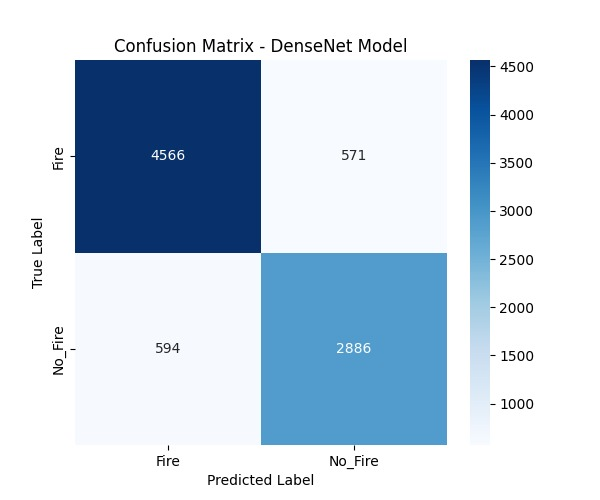
\includegraphics[width=0.45\textwidth]{densenet}
    \quad
    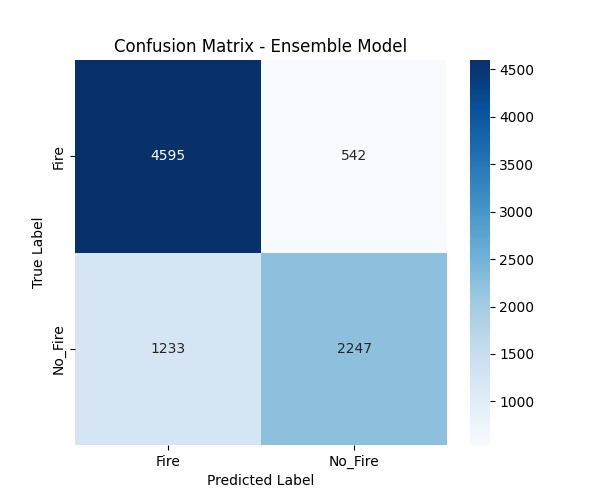
\includegraphics[width=0.45\textwidth]{ensemble}
    \caption{DenseNet (left) vs. Ensemble (right) confusion matrices.}
    \label{fig:confmat}
\end{figure}

DenseNet shows fewer false negatives, making it appealing for early fire detection,
while the ensemble yields a more balanced classification in certain scenarios.
